\Section{The Goman and Khrabrov model}

\Subsection{Motivation}
In their 1994 paper entitled ``State-Space Representation of Aerodynamic Characteristics of an Aircraft at High Angle of Attack'' \cite{GK} Goman and Khrabrov introduce a new model for characterizing the lift and moment coefficients for slender delta wings.
Their goal was to study the stability of delta wing fighter jets where maneuverability is important, and to link it to physical fluid dynamic phenomenons such as vortex breakdown or flow separation.

\par The classical stability analysis method relies on a Taylor series expansion of the aerodynamic coefficients.
% maybe put an example here.
This linear representation is relatively accurate for fully attached flow but the model breaks down at higher angle of attack when separation occurs.
In the semi separated region the aerodynamic effects are mainly driven by the degree of flow separation happening on the wing.
For this reason they chose to define $C_l$ as a function of $\alpha$, the angle of attack, and a state variable $x$ representing the degree of separation.
This degree of separation can be defined as the position of the vortex breakdown point if you are looking at delta wings, or the position of the reattachment point in the case of 2D airfoils.
This allows for a model tightly defined by the physics of the flow.


\Subsection{Flow physics and state variables}
Since this study was performed with a 2D NACA0009 airfoil, we define the state variable $x$ as the position of the reattachment point.
Its value linearly change from 1 when it is situated at the leading edge to 0 when it gets to the trailing edge and beyond.
For quasi-steady cases separation point is a function of the angle of attack. If we define $x_0$ as the separation point position in a quasi-steady situation then

\begin{equation}
  C_l^{qs} = f(\alpha,x_0(\alpha))
  \label{eqn:qs_Cl}
\end{equation}

The unsteady part of the flow physics can be divided into two groups of phenomenons.

\par The firsts are the effects of the angle of attack variation speed on the position of the separation point.
Goman and Khrabrov argue that this is roughly proportional to the pitch rate $\dot{\alpha}$ and as such they can be included by modifying the quasi-steady state value by using $x_0 (\alpha - \tau_2 \dot{\alpha})$ 

\par The second phenomenon is due to the dynamics of the separated flow.
The flow has a certain relaxation characteristic under a disturbance input.
This can be modeled using a first order differential equation.

\begin{eqnarray}
  \tau_1 \frac{dx}{dt} +x = x_0(\alpha - \tau_2 \dot{\alpha}) 
  \label{eqn:state_variable}
\end{eqnarray}



\Section{Experimental Setup}

\Subsection{Equipment and facilities}

\begin{figure}[h]
  \begin{center}
		%\includegraphics{<+file+>}
  \end{center}
  \caption{Airfoil model inside the wind tunnel}
  \label{fig:wind_tunnel}
\end{figure}

All of the experimental part of this research was performed into the Andrew Fejer Unsteady Wind Tunnel at the Illinois Institute of Technology, Chicago.
This is a low velocity wind tunnel with a 60cm by 60cm test section.
The wind tunnel is mainly used for unsteady aerodynamic studies.
Airfoils are mounted on a motorized sting outfitted with two linear electric servo-motors.
These servos are powered by an amplifier with a integrated PID system and driven by an analog voltage input signal proportional to the desired position.

\begin{figure}[h]
  \begin{center}
%		\includegraphics{<+file+>}
  \end{center}
  \caption{Pitching and plunging mechanism}
  \label{fig:pitching_mechanism}
\end{figure}

As seen on figure \ref{fig:pitching_mechanism} combining the motion of the front and back servo allows for the wing to be plunged as well as pitched around a range of axis.
The tunnel is also equipped with a system of shutters that can be used to create wind gusts.
However this feature will not be used in this project.

\par The input signal for the servos is made with Simulink\textsuperscript{\textregistered} and fed through D-Space\textsuperscript{\textregistered} as an analog voltage.

\par Several sensors are used for data acquisition.
A pair of linear potentiometers measures the position of the servos in order to get the airfoil pitch angle.
The flow speed is measure via a Pitot tube and pressure transducer plugged into a acquisition box.
In parallel to this acquisition box the forces exerted on the airfoil can be measured.
A piezoelectric ATI Nano17 force balance seats between the sting and the airfoil.
This sensor measures both absolute forces and moments along 3 different axis.

\par The wing is made out of balsa wood with a 3D printed leading edge housing the active flow control system.
This system will be described in more detail in the appropriate chapter.
The structure is wrapped in mono-coat, a heat-shrunk plastic film.
Its chord length is 245mm its width 560mm with a NACA0009 profile.
It connects to the force balance at a point at 25 percent of the chord.
The maximum was made to keep the weight and moment of inertia as small as possible to minimize the inertial effects when the wing is moving.


\FloatBarrier

\Subsection{Experimental procedure and data processing}
Different pitch input have been tried.
There was some fears at first that if the pitching axis wasn't on the axis symmetry, at the quarter chord of the airfoil, additional aerodynamic phenomenon would affect the data.
After testing different pitching input that placed the rotation axis either at the top of the front servo, at the top of the force balance or at the top of the back servo,  it was determined that the optimal way to drive the pitching mechanism was to move only the back servo.
Other input method induced to much mechanical vibrations and did not seems to make any difference aerodynamically.

\par The amplifier driving the electric servos has its own PID control system, however even after careful tunning some error exists between the commanded angle of attack and the actual angle of attack.
To negate that effect the actual servo position, as given by the potentiometers, is used for our measurements.
This data is used to transform the normal and tangent force into lift and drag (via a simple rotation matrix). 
They are then normalized to get the aerodynamics coefficients.

\par Unless specified otherwise, all the acquisitions have been done at a flow speed of 3m/s which correspond to a Reynolds number of 50000.

\par For each experimental case the force balance as well as the servo position and a synchronization signal are simultaneously acquired.
A first offset with the tunnel off and the wing pitching is taken to let us get the force balance offset as well as record the inertial effects.
Even tho the wing is only weighing around 300 grammes, these inertial effects represent the majority of the forces measured by the force balance.
Moreover some of the force measured come from the springiness of the cables used for the active flow control part.
After the first offset the real case is taken, followed by a second offset to account for the drift in the force balance measurement sometime seen over the course of several minutes.

\par During each acquisitions at least 50 cycles are recorded.
This allows us to perform what we call phase averaging.
This is done by slicing the files into individual cycles (thank to the synchronization signal) and then making an average of these cycles.
With this technique the signal to noise ratio of greatly improved.
Once this has been done with the 2 offsets and the proper acquisition itself, aerodynamic forces are obtained by subtracting the offsets.
All this processing is done with Matlab\textsuperscript{\textregistered}. 

\par The servo actuation system has a small but noticeable dead band as well as a delay between the input and output.
This makes the actual pitching motion slightly different from the input.
To account for that the actual measured pitch angle is used as an input of the GK model when we want to compare its prediction with the experimental data.

\par Finally the GK model itself is also implemented in Matlab.
The code can be seen in annex \ref{ch:GK_code}.



\FloatBarrier

\Section{Model validation}

\par While the ability to predict lift and drag based on separation can be useful, the real strength of the GK model resides in its ability to work on unsteady cases.
The first step is to determine the 2 $\tau$ time constants. 
To do that a series of pitching cases are performed. 
The pitching inputs are the following

\begin{equation}
	\alpha\left( t \right)= A \sin \left( 2 \pi \frac{t}{f} \right) + \alpha_0
	\label{eqn:pitch_input}
\end{equation}

With $A=2^\circ$ and $\alpha_0=12^\circ$.
The frequency $f$ is set to 0.25, 0.5, 1 and 2 Hz (respectively K of 0.064, 0.128, 0.257 and 0.513)

\begin{figure}[h]
  \begin{center}
    \scalebox{0.8}  
    {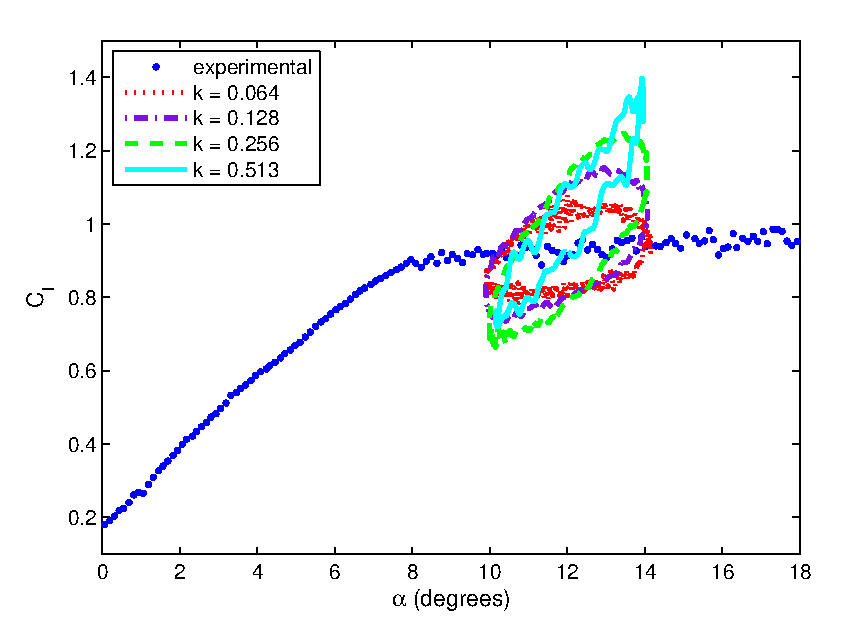
\includegraphics{./Figures/Pitching_allcases_CL_12_amp_2.eps}}
  \end{center}
  \caption{Unsteady effects on the lift of sinusoidal pitching around 12 degree} 
  \label{fig:Pitching_allcases_Cl_12}
\end{figure}

\begin{figure}[h]
  \begin{center}
    \scalebox{0.8}  
    {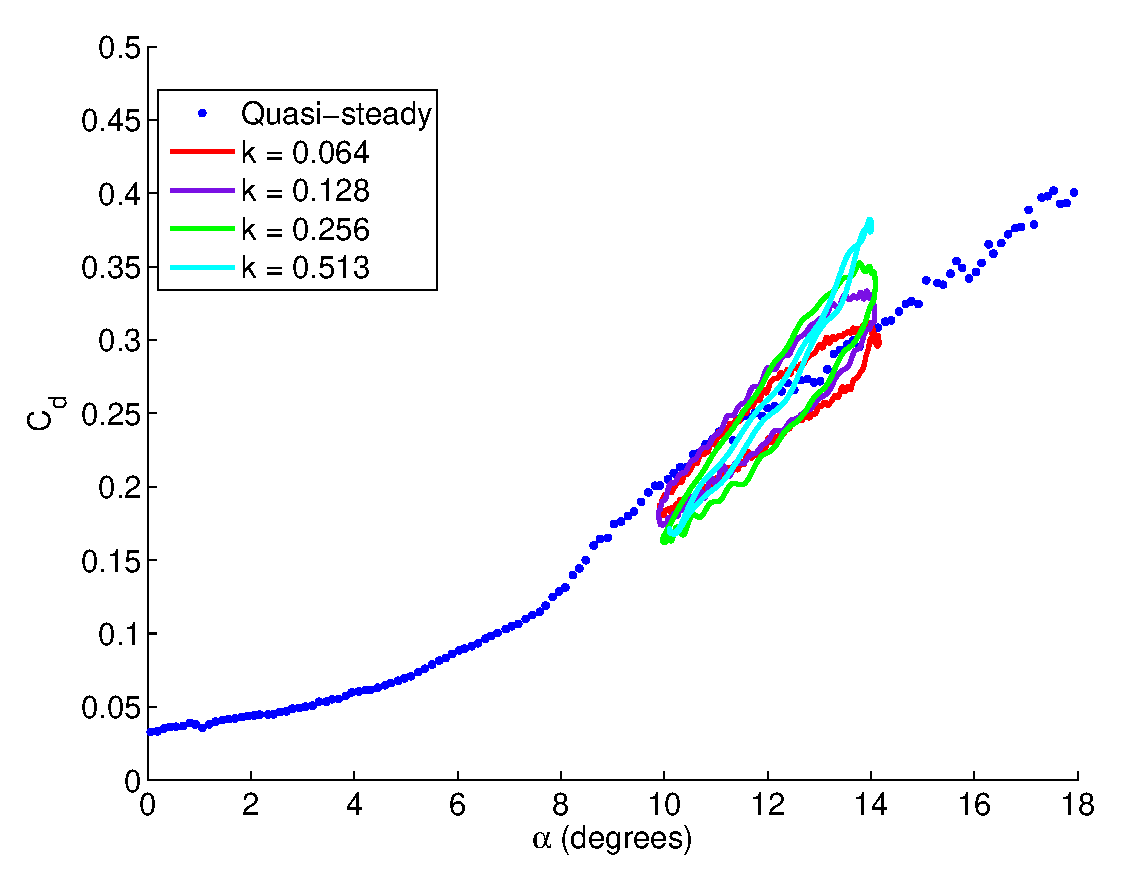
\includegraphics{./Figures/Pitching_allcases_CD_12_amp_2.eps}}
  \end{center}
  \caption{Unsteady effects on the drag of sinusoidal pitching around 12 degree} 
  \label{fig:Pitching_allcases_Cd_12}
\end{figure}

\FloatBarrier

\par On these figures it is easy to notice the influence of the time delays on the aerodynamic coefficients.
At the lower frequencies the loops are quite open and a significant difference exists between the lift obtained during the pitch up and the pitch down phase.
These lift value circulate on these loops rotating in an anti-clockwise direction.
This means that the lift is higher during pitch down maneuver.
Contrastingly this behavior disappears at higher frequencies.
For K values of 0.257 and 0.513 the difference between the pitch up and pitch down is lower.
However the lift variation amplitude is more pronounced in those cases.

\par Before using the Gk model as a predictive tool the time constants need to be found.
This is done by trial and error.
The two time constants are determined manually and are tuned to produce the best results at the different frequencies tested.
$\tau_1$ is found to be equal to 3.06 t+ (0.25s) and $\tau_2$ is 4.29 t+ (0.35s).

\par Now that the model is complete its accuracy can be checked.
The most obvious result is that the shape of the lift and drag versus angle of attack curves are similar to the experimental results.

\begin{figure}[h]
  \begin{center}
    \scalebox{0.8}{
      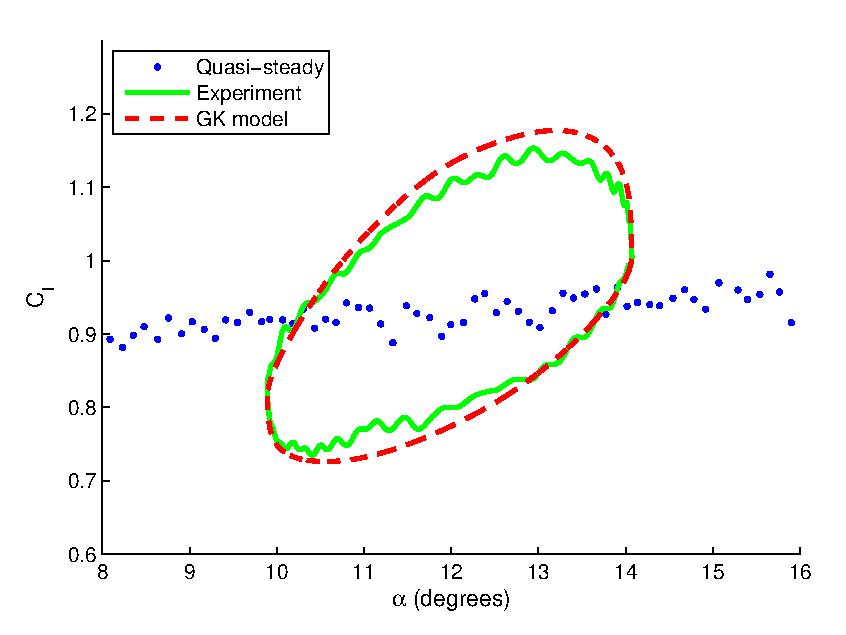
\includegraphics{./Figures/Cl_u=3_meanaoa=12_amp=2_freq=0p5.eps}}
  \end{center}
  \caption{Comparison of experimental lift coefficient and model prediction after tunning of the time constant at k =0.128}
  \label{fig:Cl_u=3_meanaoa=12_amp=2_freq=0p5}
\end{figure}

\begin{figure}[h]
  \begin{center}
    \scalebox{0.8}{
      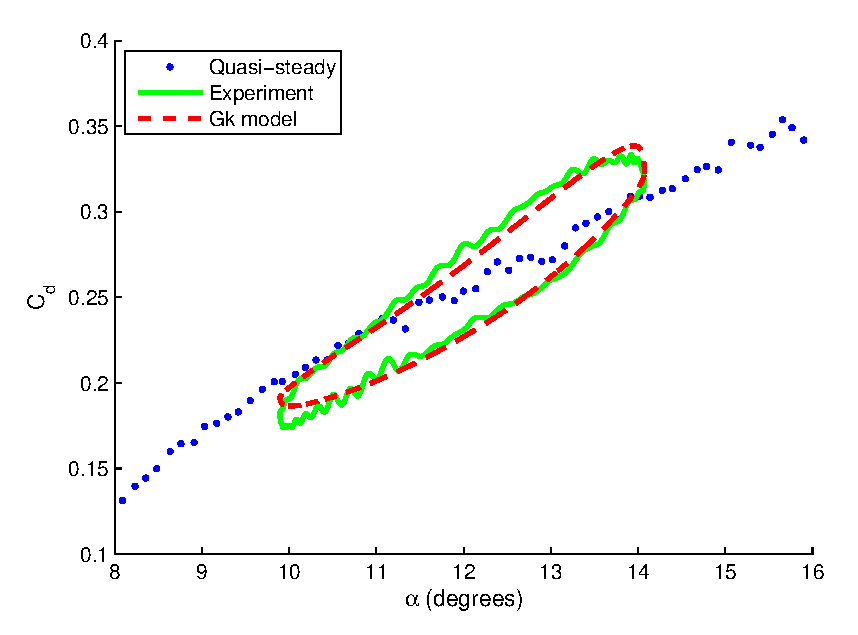
\includegraphics{./Figures/Cd_u=3_meanaoa=12_amp=2_freq=0p5.eps}}
  \end{center}
  \caption{Comparison of experimental drag coefficient and model prediction after tunning of the time constant at k =0.128}
  \label{fig:Cd_u=3_meanaoa=12_amp=2_freq=0p5}
\end{figure}

\FloatBarrier

\par This behavior can be checked for other frequencies as well.

\begin{figure}[h]
  \begin{center}
    \scalebox{0.8}  
    {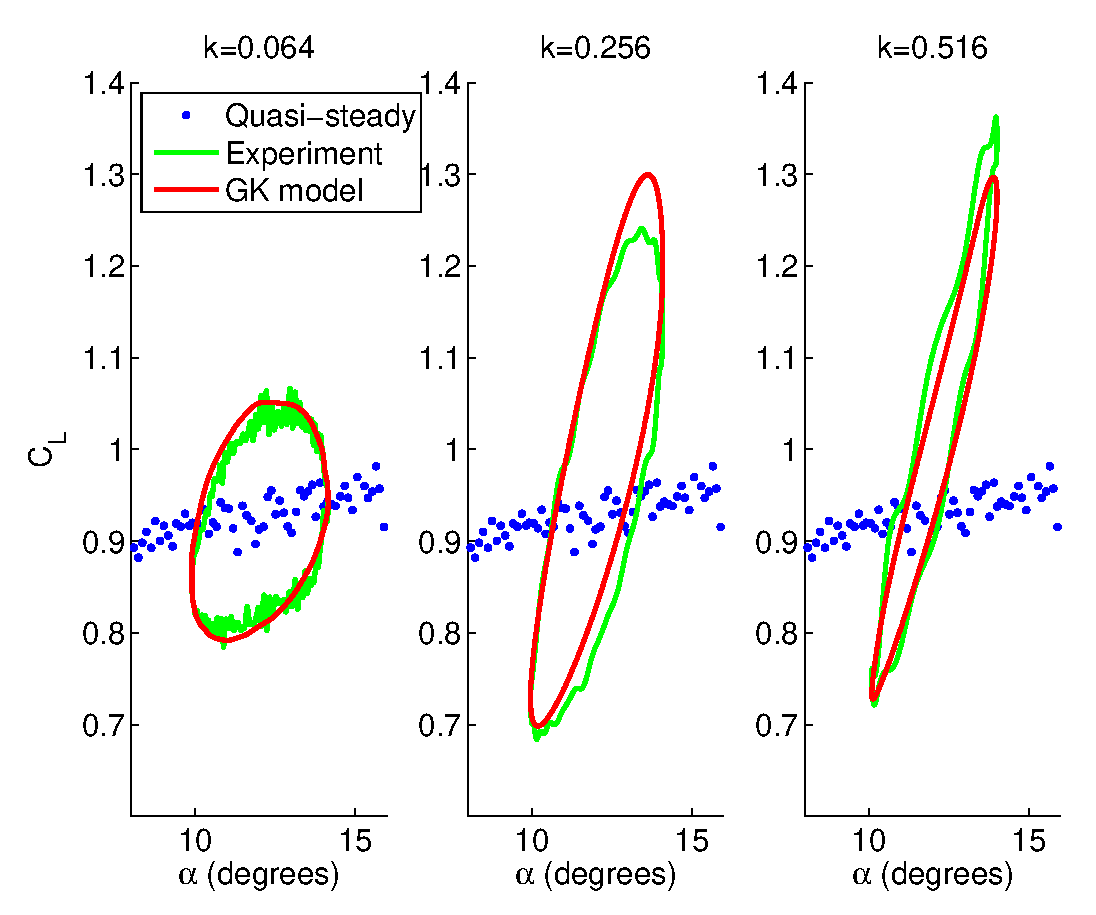
\includegraphics{./Figures/Pitching_allcases_GK_CL_12_amp_2.eps}}
  \end{center}
  \caption{Lift measurement and prediction during sinusoidal pitching around 12 degree} 
  \label{fig:Pitching_allcases_GK_Cl_12}
\end{figure}

\begin{figure}[h]
  \begin{center}
    \scalebox{0.8}  
    {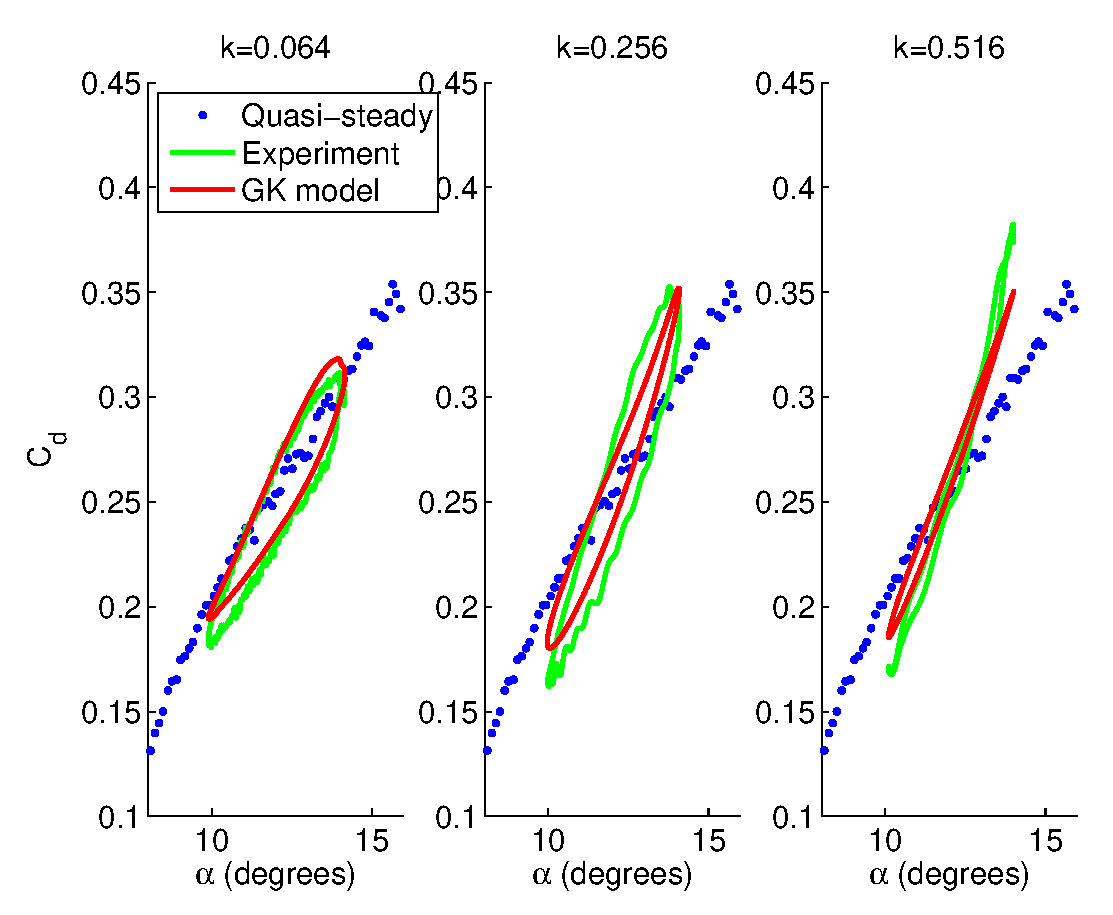
\includegraphics{./Figures/Pitching_allcases_GK_CD_12_amp_2.eps}}
  \end{center}
  \caption{Drag measurement and prediction during sinusoidal pitching around 12 degree} 
  \label{fig:Pitching_allcases_GK_Cd_12}
\end{figure}

\par Similarly another set of acquisitions is made at a mean angle of 10 degrees (see figures \ref{fig:Pitching_allcases_GK_Cl_10} and \ref{fig:Pitching_allcases_GK_Cd_10}).
The behavior is comparable at K of 0.257 and 0.513 but the drag has a noticeably different shape at K of 0.128.
For some unknown reason the model does not seems to account for the hysteresis at this frequency.

\begin{figure}[h]
  \begin{center}
    \scalebox{0.8}  
    {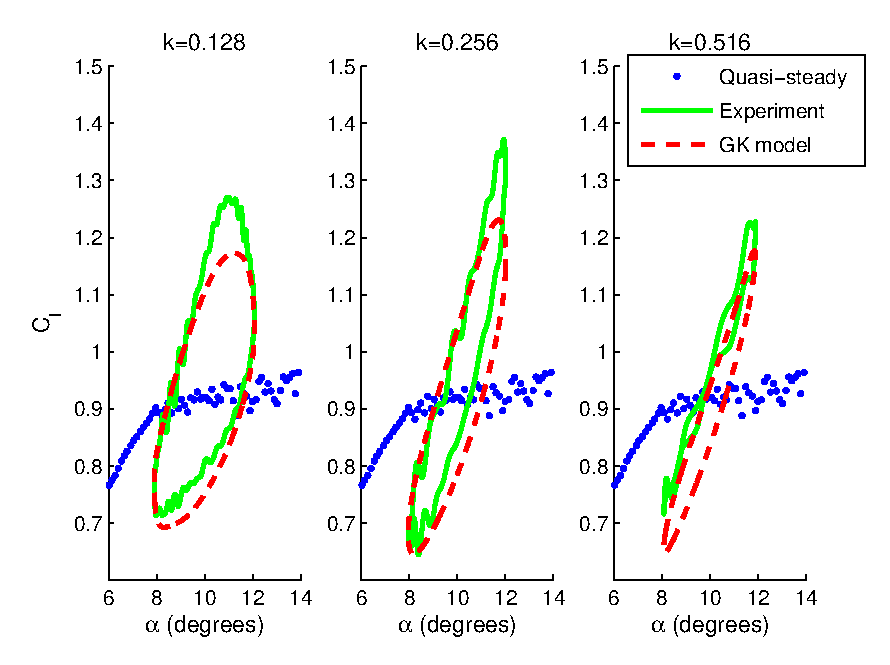
\includegraphics{./Figures/Pitching_allcases_GK_CL_10_amp_2.eps}}
  \end{center}
  \caption{Lift measurement and prediction during sinusoidal pitching around 10 degree} 
  \label{fig:Pitching_allcases_GK_Cl_10}
\end{figure}

\begin{figure}[h]
  \begin{center}
    \scalebox{0.8}  
    {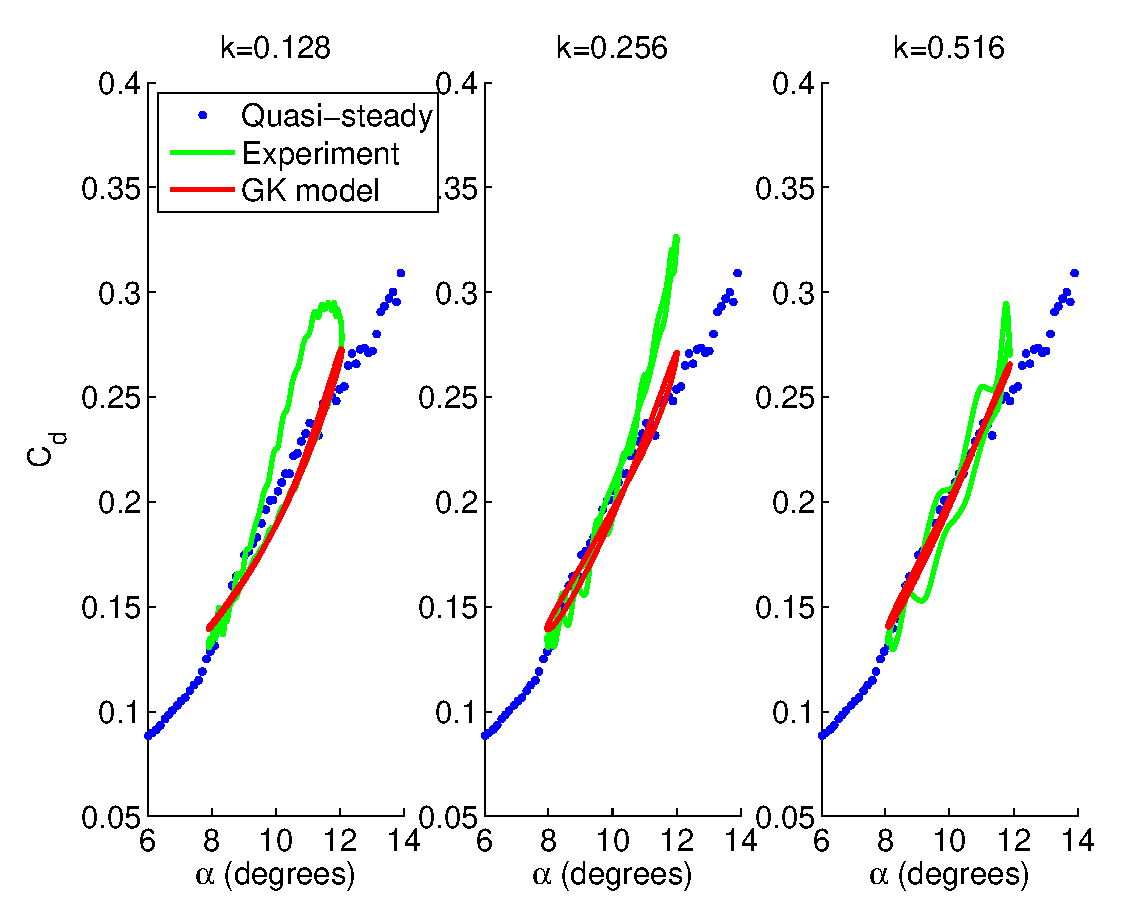
\includegraphics{./Figures/Pitching_allcases_GK_CD_10_amp_2.eps}}
  \end{center}
  \caption{Drag measurement and prediction during sinusoidal pitching around 10 degree} 
  \label{fig:Pitching_allcases_GK_Cd_10}
\end{figure}

\FloatBarrier
 %put both sinusoidal and ``random'' motion
 %Also try a non dimensional validation

\par Another obvious parameter to check for our model is the amplitude of the oscillations.
The amplitude is set to a range from 1 to 4 degrees at different mean angle of attack.
The predictions still reasonably match the experimental results. 


% divers figures

\par To simulate a more realistic pitch profile, a pseudo-random pitch profile is designed.
The input is constructed as seen in equation \ref{eqn:random_pitch_input} with a randomized phase difference $\varphi_i$ between each harmonic components.

\begin{equation}
	\alpha_{random}= \frac{\sum_{i=1}^{10} \sin (\frac{2 \pi t}{f_i} + \varphi_i)}{B} + \alpha_{0}
	\label{eqn:random_pitch_input}
\end{equation}

The frequency are regularly spaced between 0.25 and 2Hz and the constant $B$ is chosen to make sure the maximum deviation from the $\alpha_0$ value is no more than 2 degrees.
This is done so that the bandwidth of the input signal is limited.

\begin{figure}[h]
  \begin{center}
    %\scalebox{0.6}  
    %{\includegraphics{./Figures/Pitching_random_Cl_12_amp_2.eps}}
  \end{center}
  \caption{Unsteady effects of random pitching on the lift}
  \label{fig:Pitching_random_Cl_12}
\end{figure}

\begin{figure}[h]
  \begin{center}
    %\scalebox{0.6}  
    %{\includegraphics{./Figures/Pitching_random_Cd_12_amp_2.eps}}
  \end{center}
  \caption{Unsteady effects of random pitching on the drag}
  \label{fig:Pitching_random_Cd_12}
\end{figure}


\FloatBarrier

\par This model is producing accurate results that account for both the dynamic effects and the flow separation.
Moreover the procedure is light enough to be implemented into the optimization algorithm without increasing too much the computation cost
